\documentclass[a4paper, 11pt]{article}
\usepackage[utf8]{inputenc} % Change according your file encoding
\usepackage{graphicx}
\usepackage{url}

%opening
\title{Seminar Report: Opty}
\author{Maria Gabriela Valdes and Victoria Beleuta}
\date{\today{}}

\begin{document}

\maketitle

\section{Introduction}

During this lab, we implemented a transaction server using optimistic concurrency control in Erlang . Opty is a concurrency control method applied to transactional systems such as relational database management systems. It assumes that multiple transactions can complete without interfering with each other, while using data resources without acquiring locks. Before committing, each transaction checks if any other transaction has changed the entry. If it hasn't been changed the transaction can commit, if there are conflicts, the transaction rollsback and restarts.
 
\section{Work done}

We have completed the code files provided to correctly implement the algorithm. Our source code can be found in the src folder. To start the algorithm locally you have to call the function \textit{start} of module \textit{opty} with six arguments in the following order: number of clients, number of entries, number of updates, number of reads, duration of experiments and size of the subset of entries to be used by each client. It's important to emphasize that each entry subset of each client is created with different random values of the original set of entries. For example: \textit{opty:start(3,4,1,1,5,2)}. With this command the Opty algorithm will start with three clients, and a store with four entries, one write operation, one read operation, with a duration of 5 seconds and a subset of 2 entries out of the total provided.\\\\
To start the algorithm with the server and clients in different Erlang nodes you first have to start two different Erlang environments. For example:
\begin{itemize}
\item In one terminal type \textit{erl -sname optyserver}. This will represent an Erlang node name \textit{optyserver@server}.\\
\item In another different terminal type \textit{erl -sname clients}. This will represent a Erlang node name {clients@server}.\\
\end{itemize}
%
First we start the server in the node \textit{optyserver@server} with the command \textit{opty:start\_server(10)}, where 10 is the number of entries. To start the clients you have to call, in the clients node, the function \textit{start\_clients} of module \textit{opty} with seven arguments: number of clients, number of entries, number of updates, number of reads, duration of experiments, the name of the server’s node and the size of the subset of entries. For example: 
\textit{opty:start\_clients(5, 10, 1, 1, 5, optyserver@server, 3)}.\\

\section{Experiments}

\textbf{In the same machine:}\\

\textbf{i)} different number of concurrent clients in the system;\\

We ran the following commands to see how the algorithm runs:
\begin{itemize}
\item opty:start(1,10,1,1,5,3)\\\\
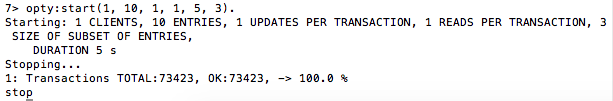
\includegraphics[scale=0.5]{images/exp-i-1.png} \\
\item opty:start(5,10,1,1,5,3)\\\\
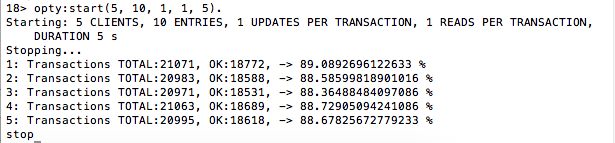
\includegraphics[scale=0.5]{images/exp-i-2.png} \\
\newpage
\item opty:start(10,10,1,1,5,3)\\\\
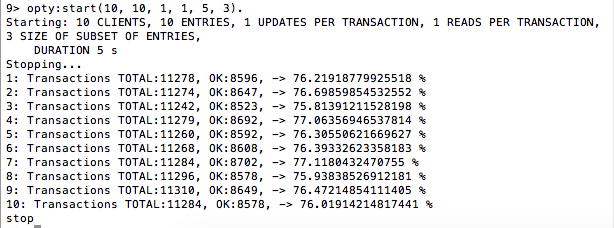
\includegraphics[scale=0.5]{images/exp-i-3.png} \\
\item opty:start(20,10,1,1,5,3)\\\\
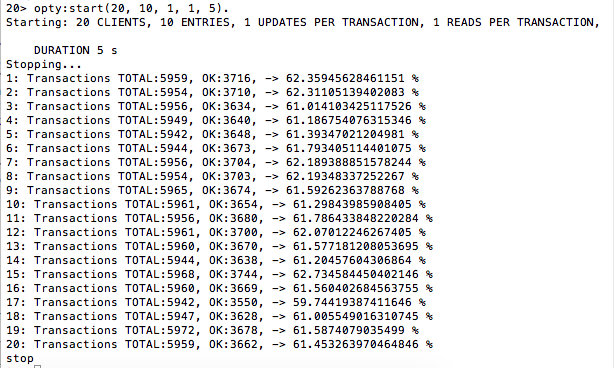
\includegraphics[scale=0.5]{images/exp-i-4.png} \\
\newpage
\item opty:start(40,10,1,1,5,3)\\\\
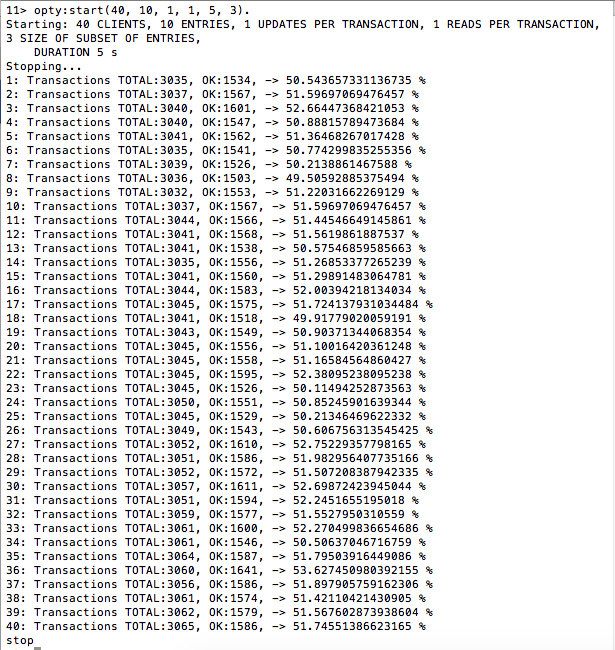
\includegraphics[scale=0.5]{images/exp-i-5.png} \\
\newpage
\item opty:start(80,10,1,1,5,3)\\\\
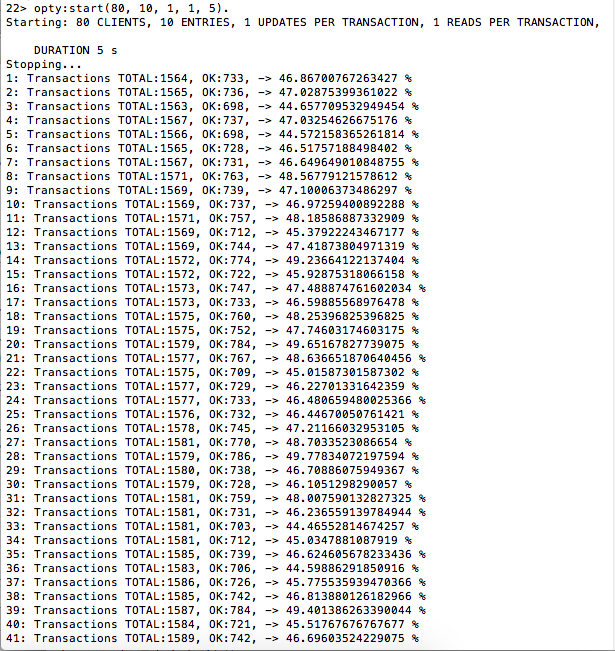
\includegraphics[scale=0.4]{images/exp-i-6a.png} \\
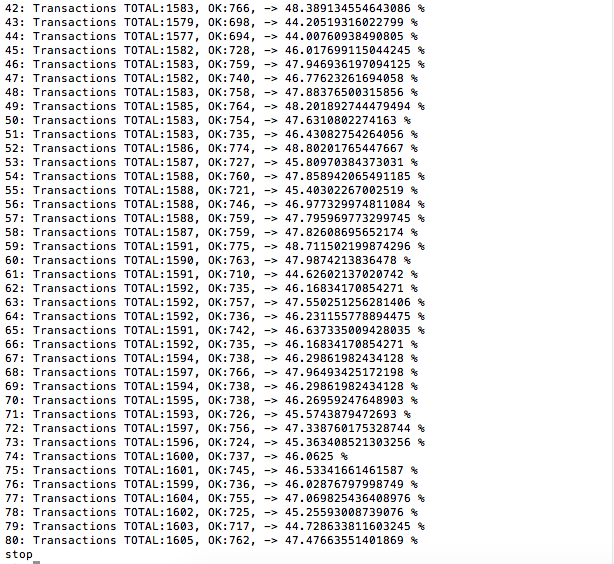
\includegraphics[scale=0.4]{images/exp-i-6b.png} \\
\end{itemize}
\newpage
%
\textbf{ii)} different number of entries in the store;\\\\
We ran the following commands to see how the algorithm runs:\\
\begin{itemize}
\item opty:start(5,1,1,1,1,1)\\\\
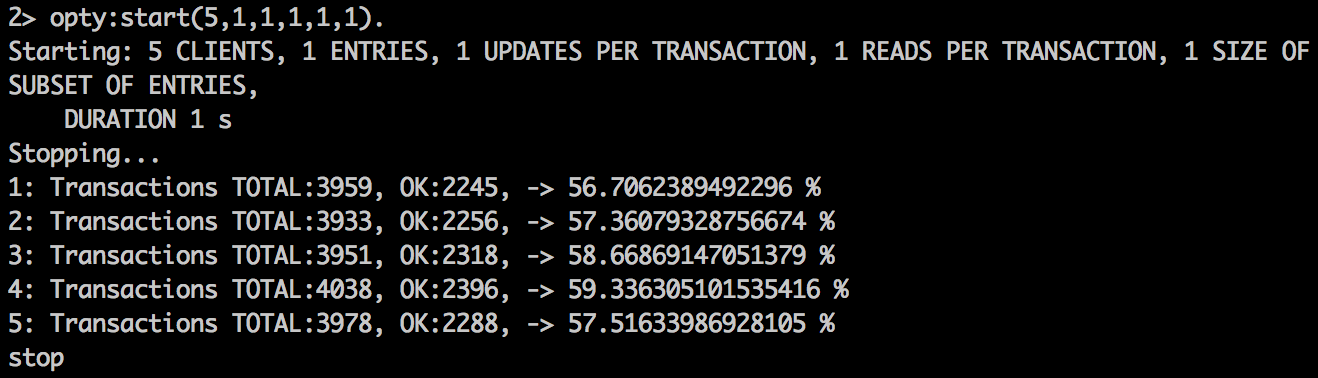
\includegraphics[scale=0.5]{images/exp-ii-1.png} \\
\item opty:start(5,3,1,1,1,3)\\\\
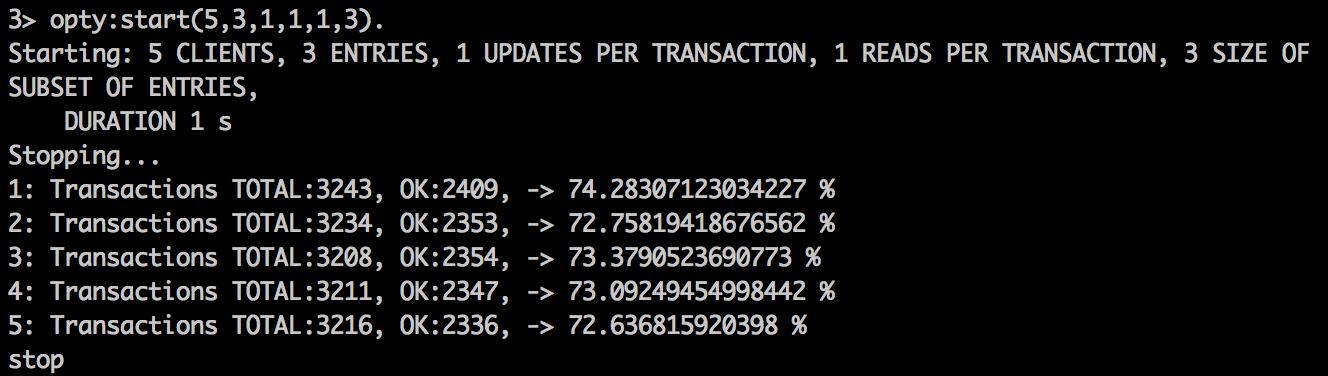
\includegraphics[scale=0.5]{images/exp-ii-2.png} \\
\item opty:start(5,5,1,1,1,5)\\\\
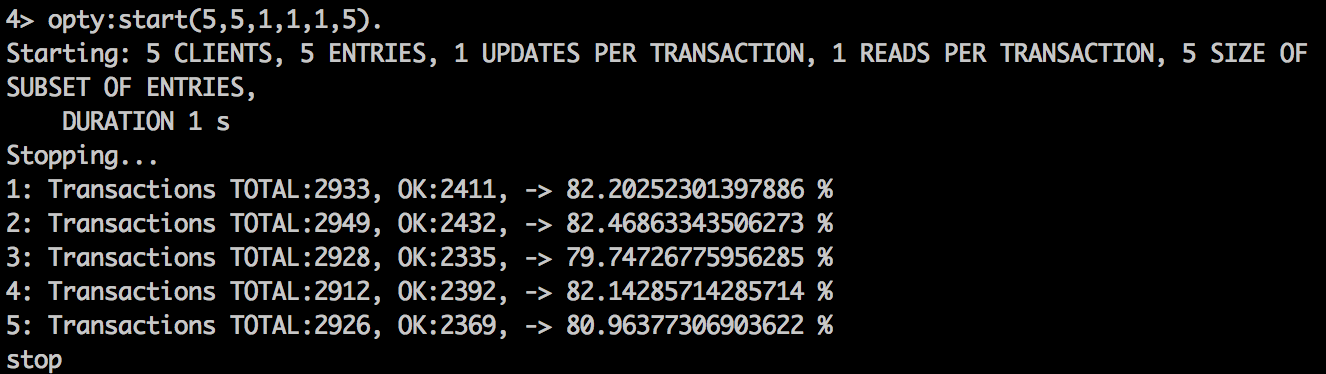
\includegraphics[scale=0.5]{images/exp-ii-3.png} \\
\newpage
\item opty:start(5,10,1,1,1,10)\\\\
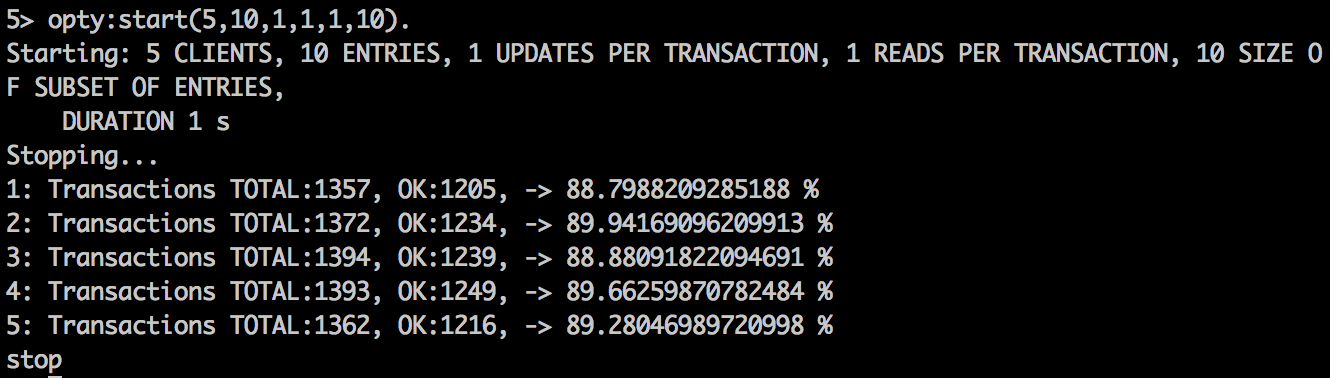
\includegraphics[scale=0.5]{images/exp-ii-4.png} \\
\item opty:start(5,100,1,1,1,100)\\\\
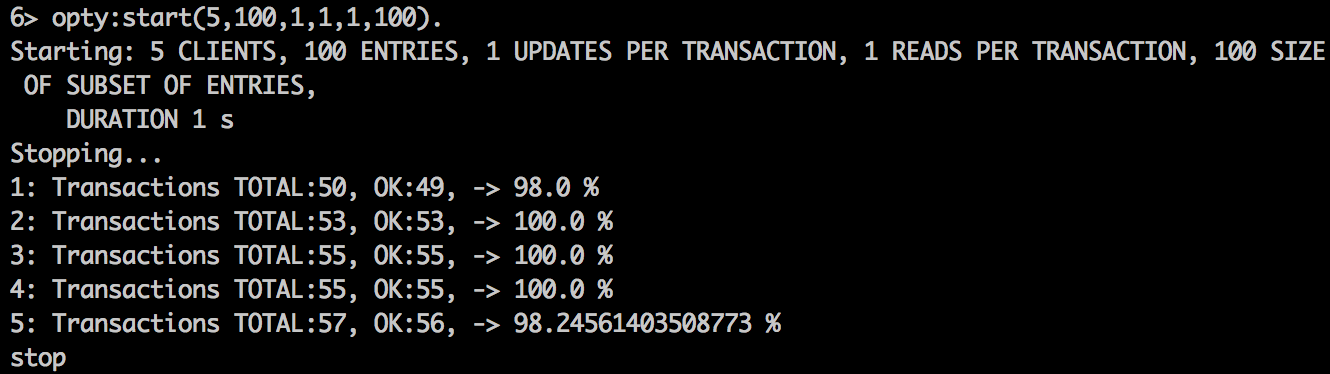
\includegraphics[scale=0.5]{images/exp-ii-5.png} \\
\item opty:start(5,1000,1,1,1,1000)\\\\
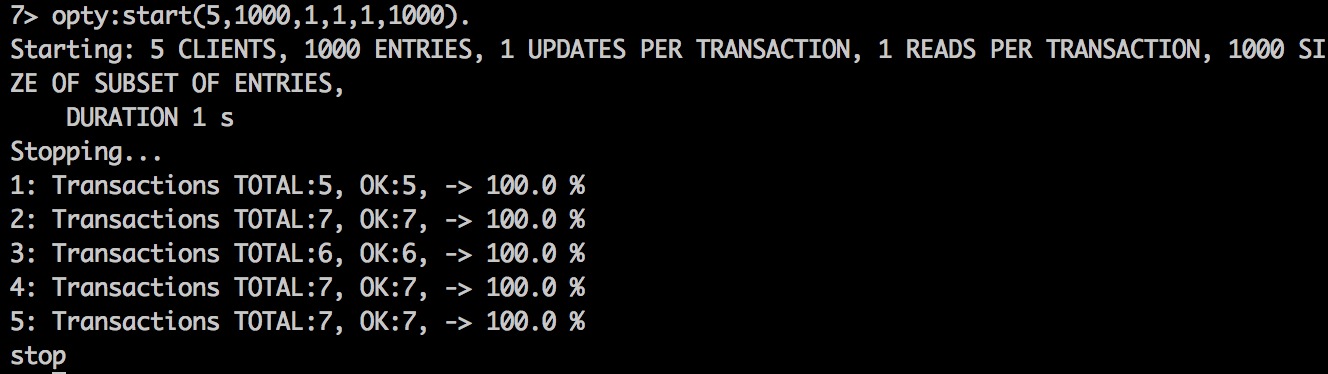
\includegraphics[scale=0.5]{images/exp-ii-6.png} \\
\end{itemize}

%
\textbf{iii)} different number of write operations per transaction;\\\\
We ran the following commands to see how the algorithm runs:\\
\begin{itemize}
\item opty:start(5,10,1,1,5,3)\\\\
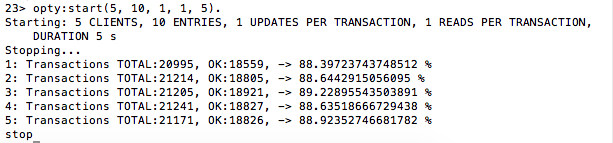
\includegraphics[scale=0.5]{images/exp-iii-1.png} \\
\item opty:start(5,10,5,1,5,3)\\\\
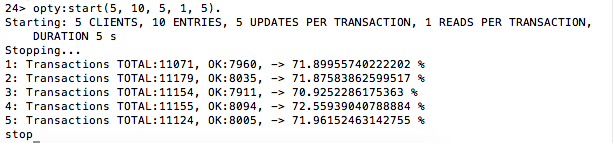
\includegraphics[scale=0.5]{images/exp-iii-2.png} \\
\item opty:start(5,10,10,1,5,3)\\\\
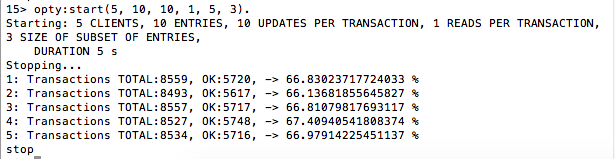
\includegraphics[scale=0.5]{images/exp-iii-3.png} \\
\item opty:start(5,10,20,1,5,3)\\\\
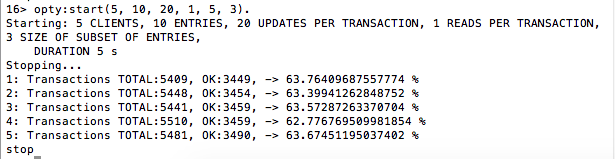
\includegraphics[scale=0.5]{images/exp-iii-4.png} \\
\item opty:start(5,10,40,1,5,3)\\\\
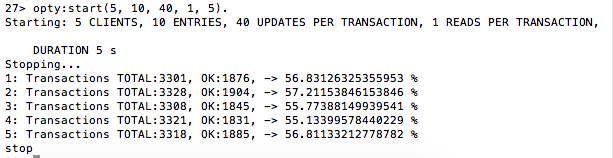
\includegraphics[scale=0.5]{images/exp-iii-5.png} \\
\newpage
\item opty:start(5,10,80,1,5,3)\\\\
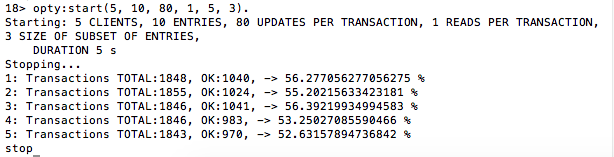
\includegraphics[scale=0.5]{images/exp-iii-6.png} \\
\end{itemize}
%

\textbf{iv)} different ratio of read and write operations per transaction;\\\\
We ran the following commands to see how the algorithm runs:\\
\begin{itemize}
\item opty:start(5,10,1,100,1,5)\\\\
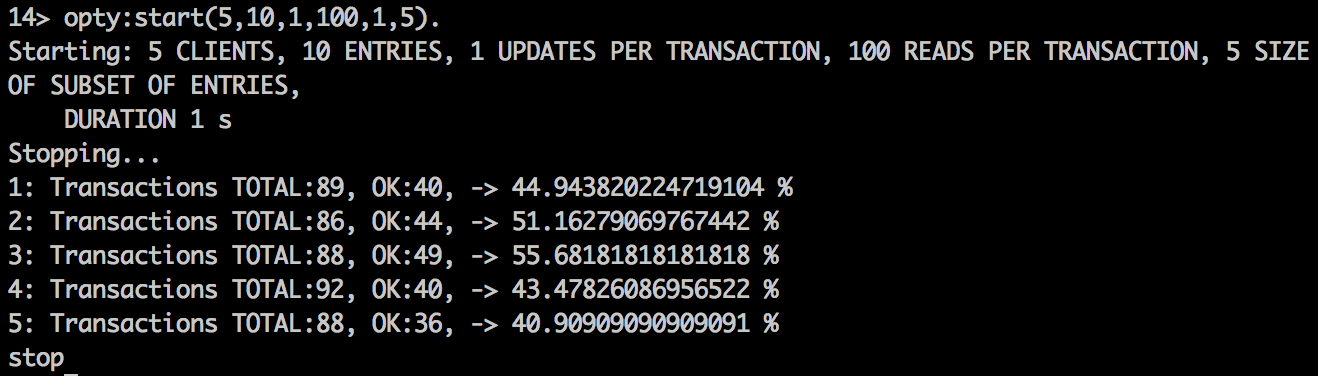
\includegraphics[scale=0.5]{images/exp-iv-7.png} \\
\item opty:start(5,10,1,10,1,5)\\\\
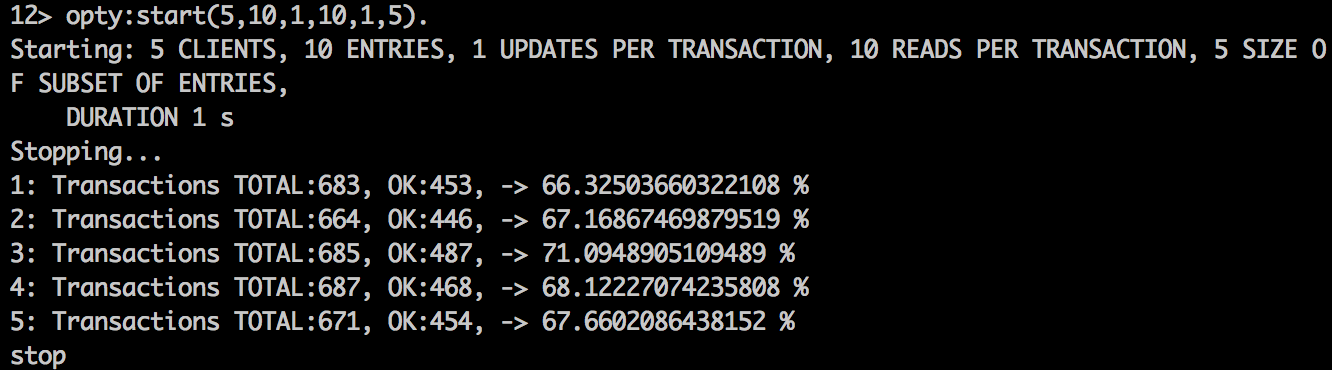
\includegraphics[scale=0.5]{images/exp-iv-5.png} \\
\item opty:start(5,10,1,3,1,5)\\\\
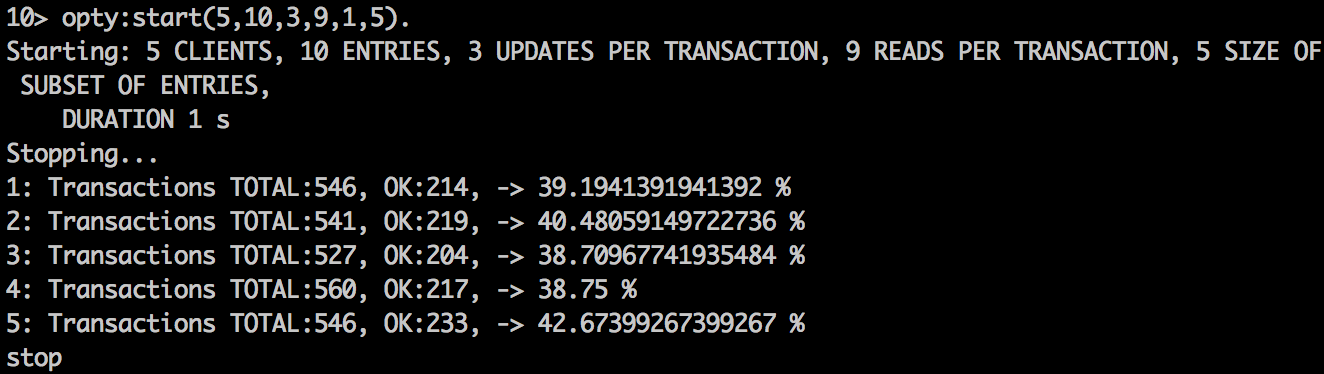
\includegraphics[scale=0.5]{images/exp-iv-3.png} \\
\item opty:start(5,10,1,2,1,5)\\\\
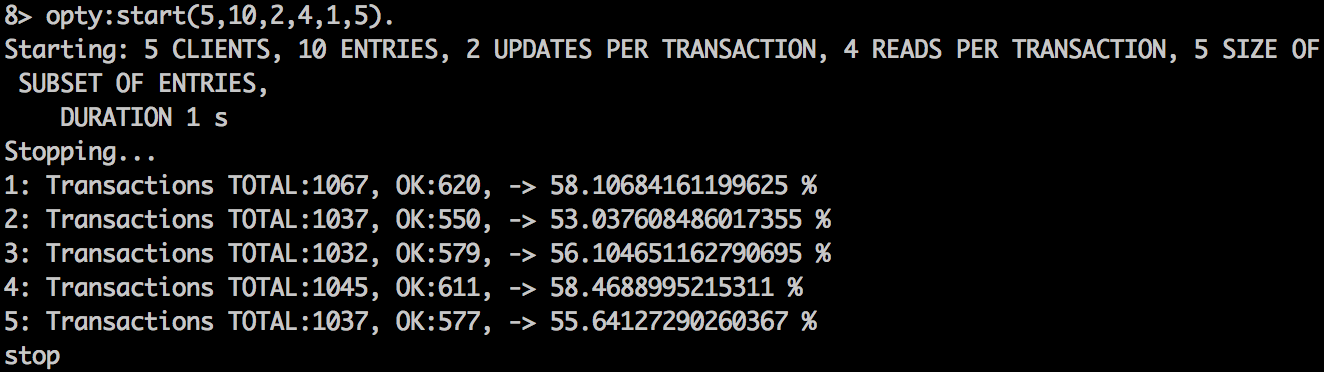
\includegraphics[scale=0.5]{images/exp-iv-1.png} \\
\item opty:start(5,10,2,1,1,5)\\\\
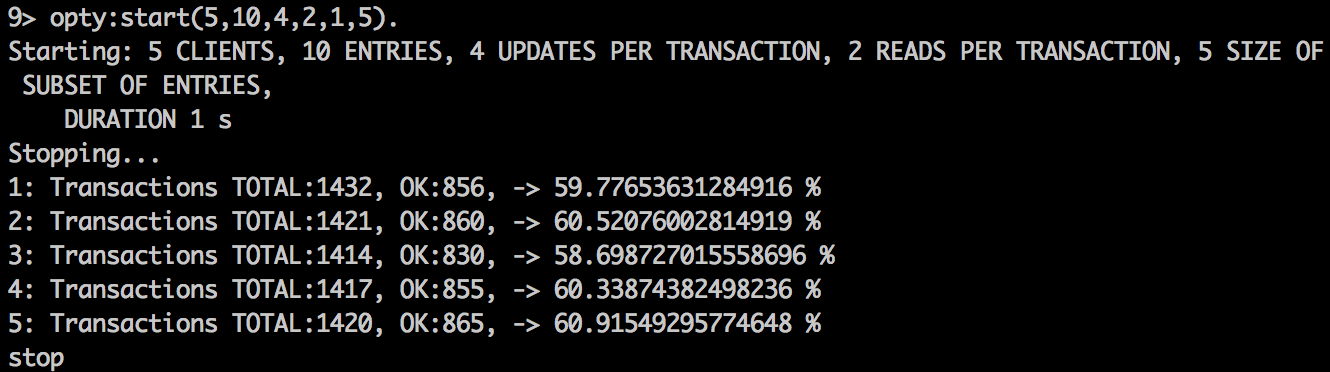
\includegraphics[scale=0.5]{images/exp-iv-2.png} \\
\item opty:start(5,10,3,1,1,5)\\\\
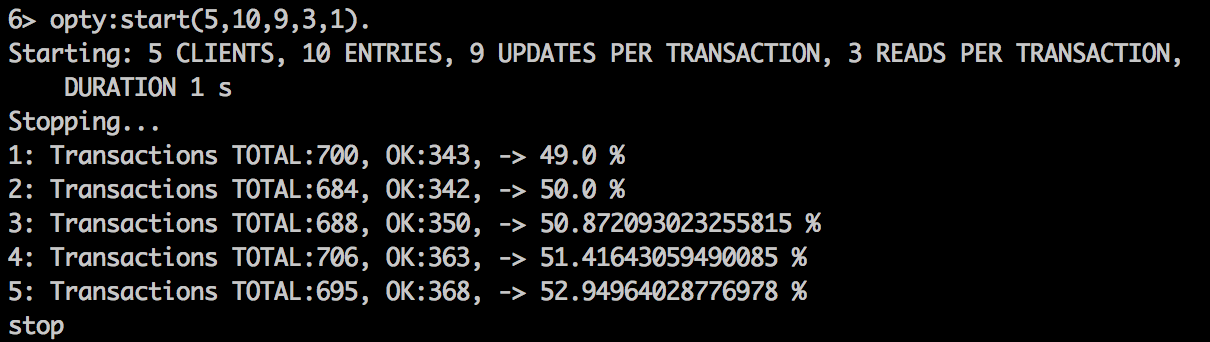
\includegraphics[scale=0.5]{images/exp-iv-4.png} \\
\item opty:start(5,10,10,1,1,5)\\\\
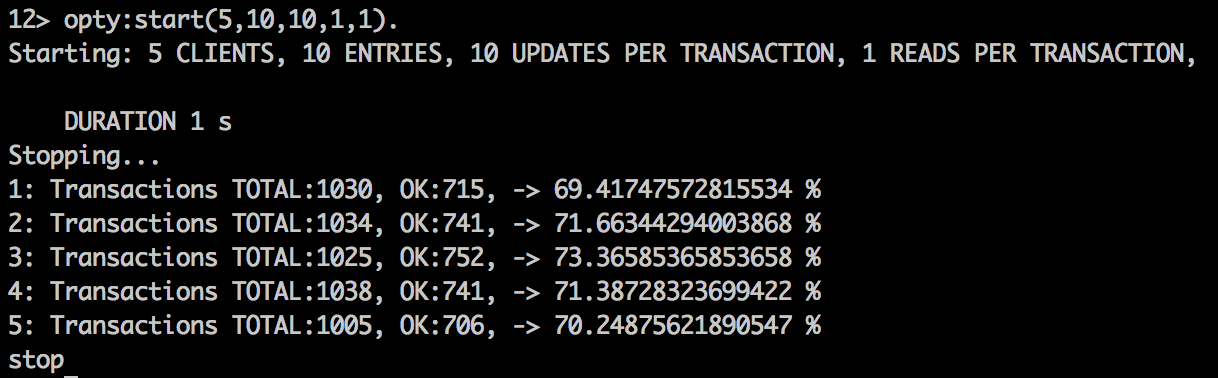
\includegraphics[scale=0.5]{images/exp-iv-6.png} \\
\item opty:start(5,10,100,1,1,5)\\\\
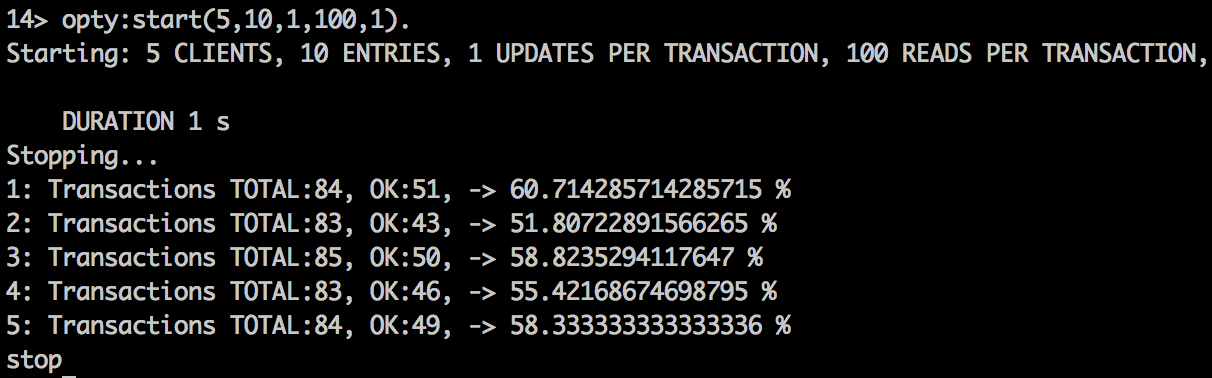
\includegraphics[scale=0.5]{images/exp-iv-8.png} \\
\end{itemize}

\textbf{v)} different percentage of accessed entries with respect to the total number of entries;\\\\

We ran the following commands to see how the algorithm runs:\\

\begin{itemize}
\item opty:start(5,10,2,2,1,2)\\\\
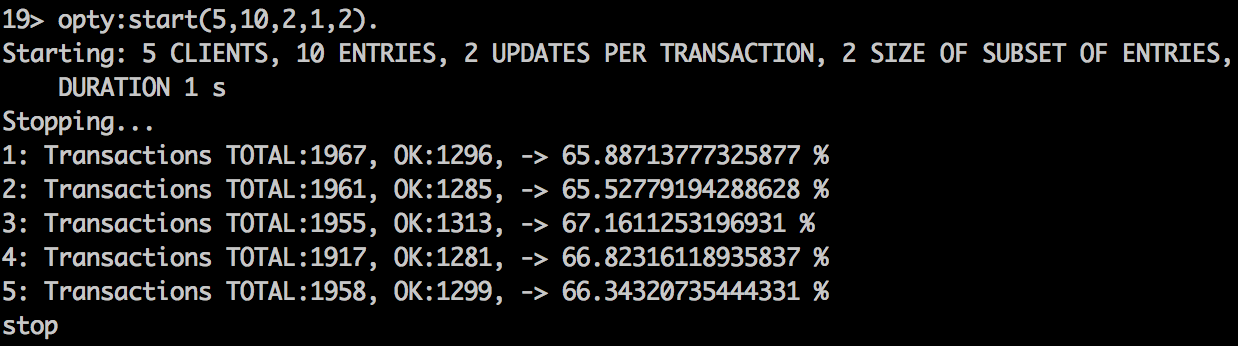
\includegraphics[scale=0.5]{images/exp-v-1.png} \\
\item opty:start(5,10,2,2,1,3)\\\\
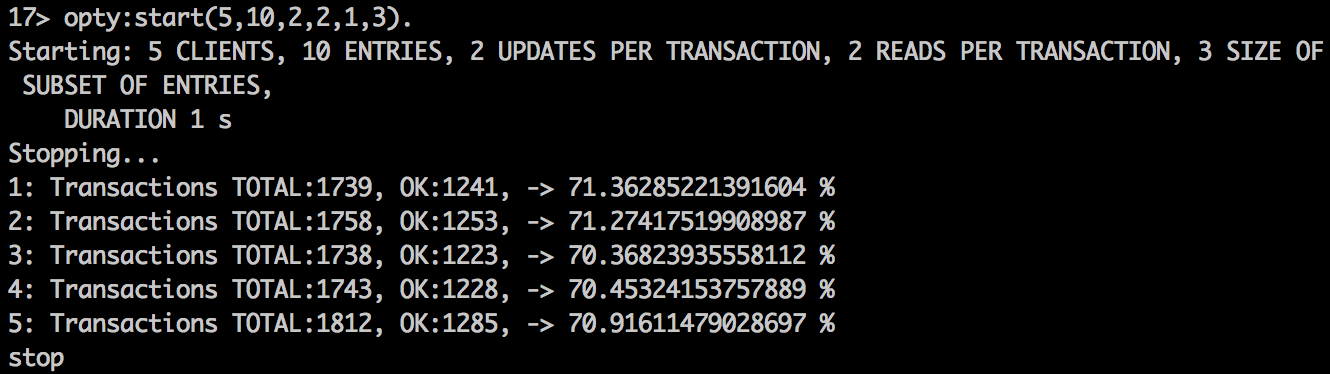
\includegraphics[scale=0.5]{images/exp-v-2.png} \\
\newpage
\item opty:start(5,10,2,2,1,4)\\\\
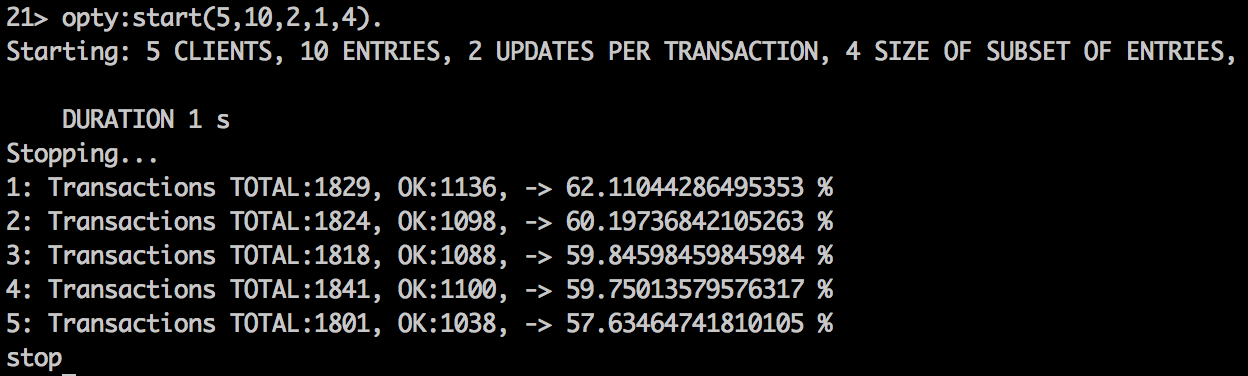
\includegraphics[scale=0.5]{images/exp-v-3.png} \\
\item opty:start(5,10,2,2,1,5)\\\\
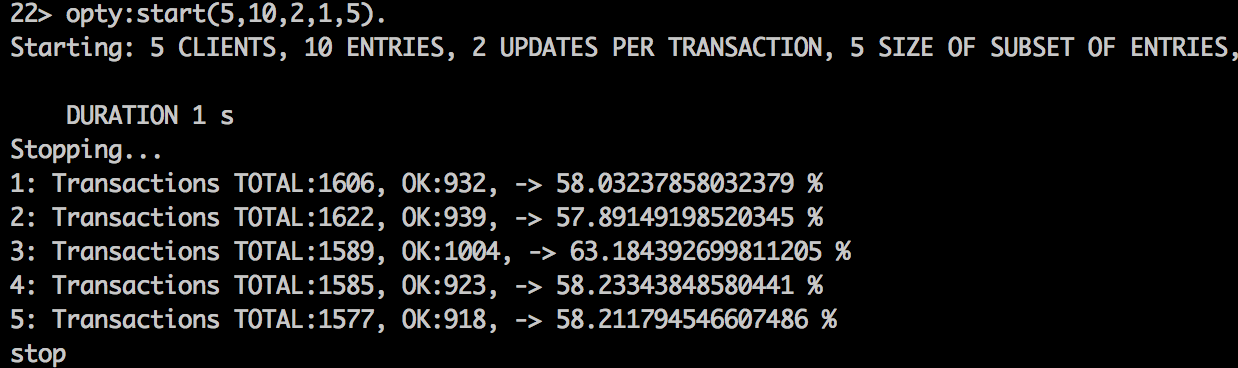
\includegraphics[scale=0.5]{images/exp-v-4.png} \\
\item opty:start(5,10,2,2,1,8)\\\\
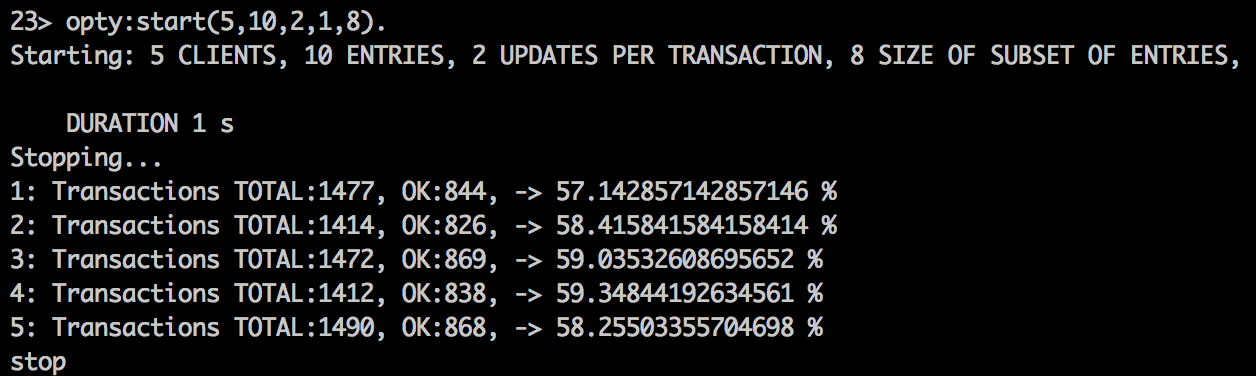
\includegraphics[scale=0.5]{images/exp-v-5.png} \\
\end{itemize}

\newpage
\textbf{In different machines:}\\\\

We created the server node: optyserver@localhost and ran the command \textit{opty:start\_server(10)}. Then we created the clients node: clients@localhost and ran the command \textit{opty:start\_clients(5, 10, 1, 1, 5, optyserver@server, 3)}.\\\\
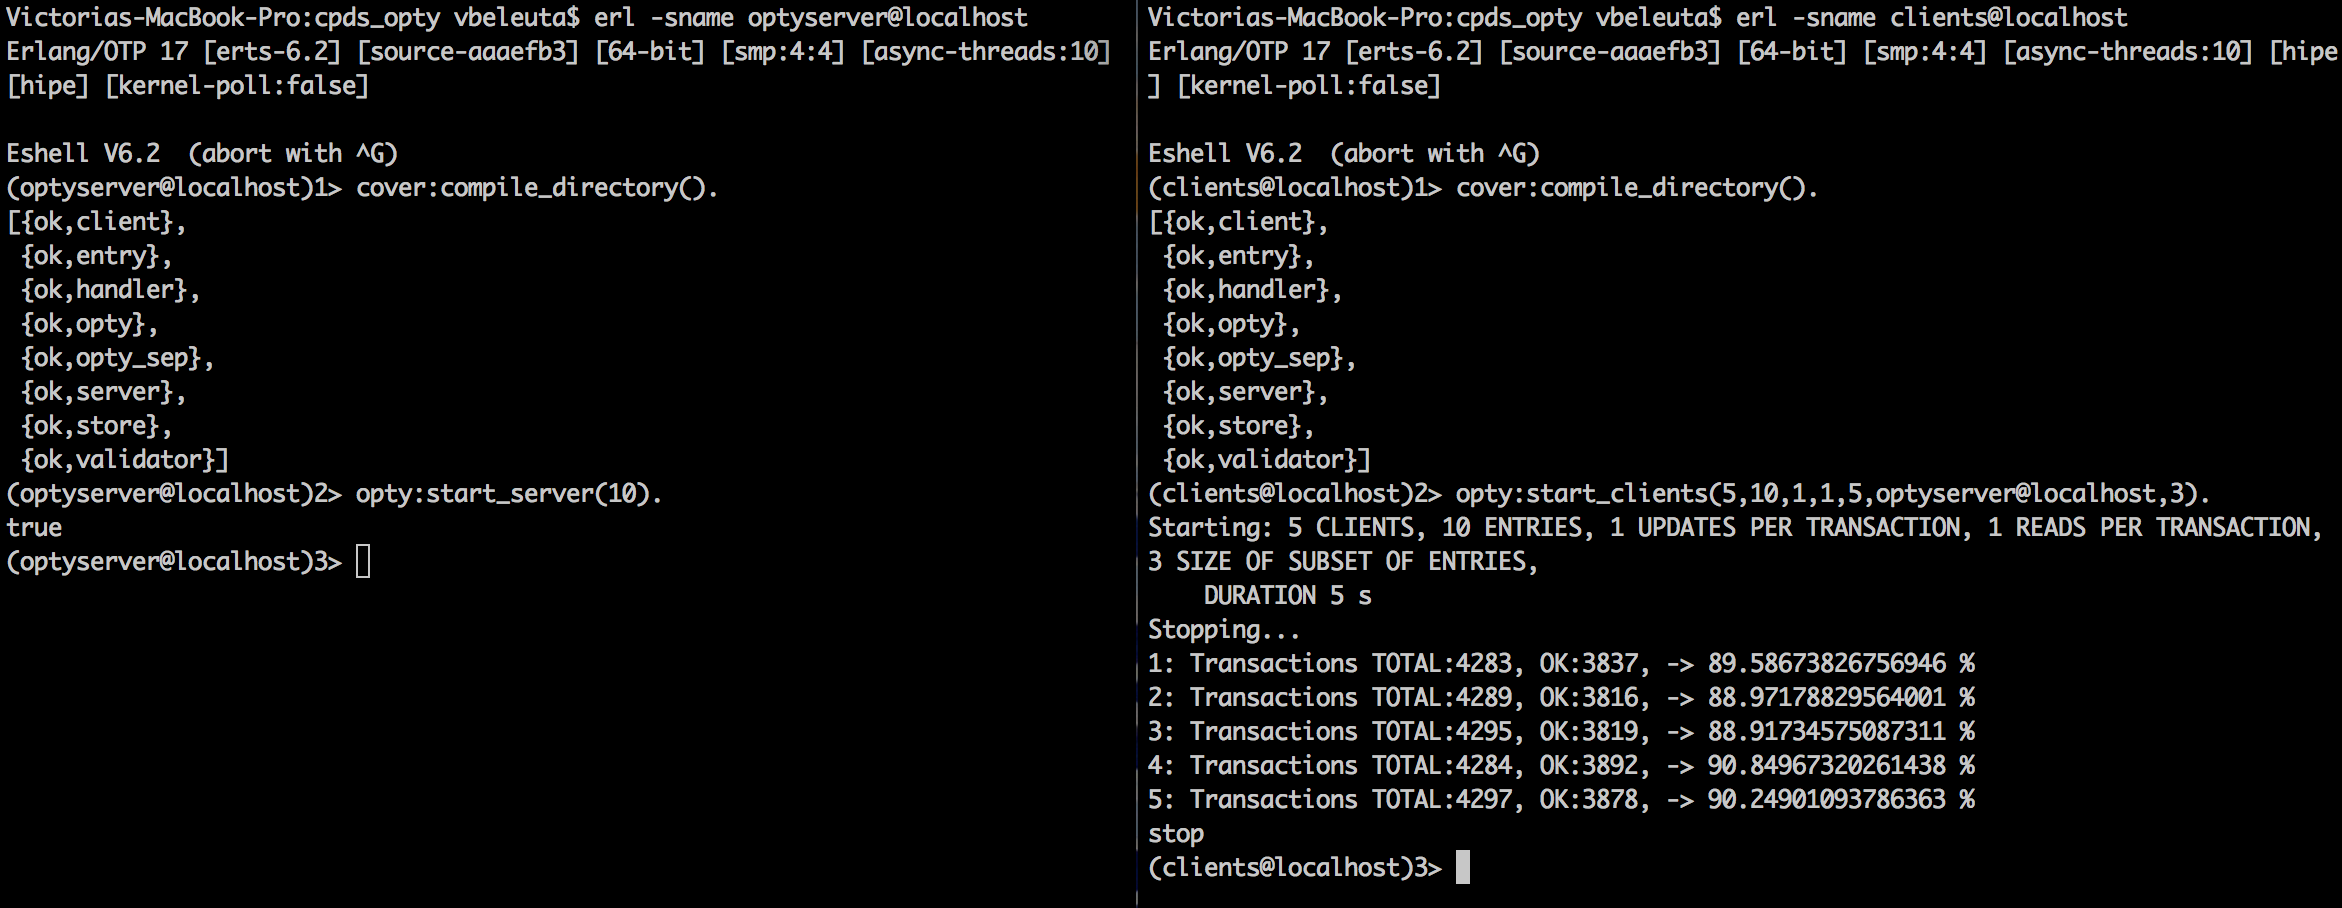
\includegraphics[scale=0.29]{images/distributed.png} \\\\

\section{Open questions}

\textbf{1)} What is the impact of each of these parameters on the success rate? Is the success rate the same for the different clients?\\

The success rate is influenced by all of these paramenters:\\
\begin{itemize}
\item For the experiment \textit{i} we see that as we increase the number of clients, the success rate decreases. This happens because as the number of clients increases, the likelihood that this clients have very similar or even equal subset of entries increases as well, and this of course, increases the number of possible conflicts to arise, increasing as well the number of aborted transactions, and as a consequence the number of non conflicting transactions decreases.\\

\item For the experiment \textit{ii} however, we see that as we increase the number of entries, the success rate also increases. This happens because with a small number of entries to work with, the likelihood of having conflicts increases because the clients share a very similar subset of entries, and as a consequence this arises more conflicts between their transactions and more aborted transactions. With a bigger entry set to share between several clients, it is more likely that each client will have different subsets of entries to work on and less number of conflicting or aborting transactions.\\

\item For experiment \textit{iii} as expected the more write operations we try to perform the more conflicts arrise forcing transactions to restart and their success rate decreases.\\

\item For experiment \textit{iv} we notice that if as we increase the nr of reads to the nr of writes, the success rate decreases (for 1 write we perform 2 reads with a success rate of ~81\%, while if we perform for each 1 write, 100 reads we have a success of ~45\% ) and if we increase the nr of writes to the nr of reads the success rate decreases as well (for 1 read we perform 2 writes with a success rate of ~81\%, while if we perform for each 1 read, 100 writes we have a success rate of ~45\%). We observe that the bigger the difference between the nr of reads and writes the more the success rate will decrease.\\

\item For experiment \textit{v} we can see that as the size of the client's entry subset increases, the number of conflicting transactions increases as well. This happens because with a bigger subset of entries, the likelihood of this subsets to have the same entries as other client's subset increases as well. As the size of the subset increases, each client will ``share'' and perform read and write operations in the ``same'' entry set increasing the probability of arising conflicts between their transactions.\\

\end{itemize}

%
\textbf{2)} If we run this in a distributed Erlang network, where is the handler running?\\

In a distributed network the handler runs in the clients node, because each node is responsible for creating it's own handler. Because of this, when the clients are destroyed so is the handler.\\

\newpage
\section{Personal opinion}
During this seminar we got an in depth view of how the Optimistic Concurrency Control algorithm works with backward validation, both locally and in a distributed environment. We are aware that this same algorithm could work with forward validation but it is interesting that thanks to the way in which the code was structured, such modification could be done only by modifying the \textit{validation} module. In our opinion, this lab had the right level of difficulty for this course and the amount of time available to us. \\

\end{document}